% !TEX TS-program = pdflatex
% !TEX encoding = UTF-8 Unicode

\documentclass[11pt]{article} % use larger type; default would be 10pt

\usepackage[utf8]{inputenc} % set input encoding (not needed with XeLaTeX)

%%% PAGE DIMENSIONS
\usepackage{geometry} % to change the page dimensions
\geometry{a4paper} % or letterpaper (US) or a5paper or....
\geometry{margin=1.5cm} % for example, change the margins to 2 inches all round
% \geometry{landscape} % set up the page for landscape
%   read geometry.pdf for detailed page layout information


%%%PACKAGES%%%
\usepackage{subfig} % make it possible to include more than one captioned figure/table in a single float
\usepackage{amsmath} % mathematics
\usepackage{amssymb}
\usepackage{graphicx}

%%% HEADERS & FOOTERS
\usepackage{fancyhdr} % This should be set AFTER setting up the page geometry
\pagestyle{fancy} % options: empty , plain , fancy
\renewcommand{\headrulewidth}{0pt} % customise the layout...
\lhead{}\chead{}\rhead{}
\lfoot{}\cfoot{\thepage}\rfoot{}

%%% SECTION TITLE APPEARANCE
\usepackage{sectsty}
\allsectionsfont{\sffamily\mdseries\upshape} % (See the fntguide.pdf for font help)
% (This matches ConTeXt defaults)

%%% ToC (table of contents) APPEARANCE
\usepackage[nottoc,notlof,notlot]{tocbibind} % Put the bibliography in the ToC
\usepackage[titles,subfigure]{tocloft} % Alter the style of the Table of Contents
\renewcommand{\cftsecfont}{\rmfamily\mdseries\upshape}
\renewcommand{\cftsecpagefont}{\rmfamily\mdseries\upshape} % No bold!


%%% END Article customizations


\title{Computer Vision II - Assignment 2}
\author{Group 23: Gustavo Willner 2708177, Pedro Campana 2461919, Helge Meier }
\date{}

\begin{document}
	\maketitle
Initiating the Stereo function with the ground truth yields problematic results. Interestingly, initiating the coarse2fine function with the GT works fine. Both the constant initialization (x=8) and the random initialization (uniformly [0,14]) seem to yield very similar results.  There seems to be a particular interval of $\alpha$ that work. Our best result came from a 0.05 alpha value with coarse2fine (Figure 7). But the same alpha value works terribly without coarse2fine (Figure 8).
\begin{figure}[ht]
  \centering
  \begin{minipage}[b]{0.45\textwidth}
    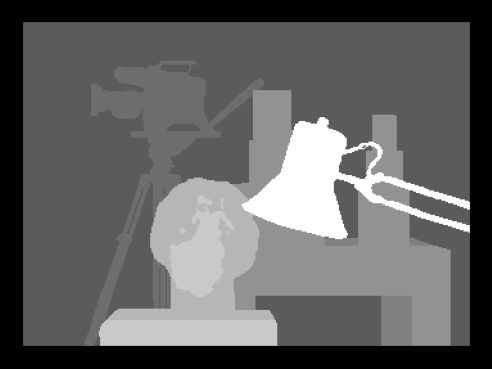
\includegraphics[width=\textwidth]{output0.png}
    \caption{Ground Truth}
    \label{fig:image1}
  \end{minipage}
  \hfill
  \begin{minipage}[b]{0.45\textwidth}
    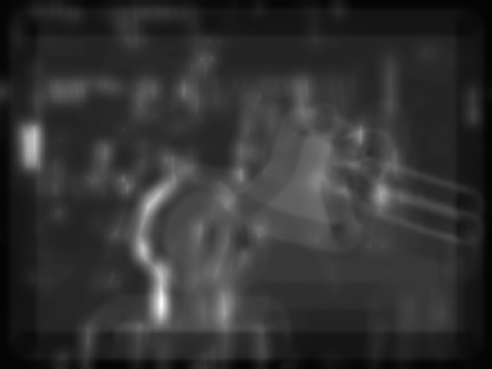
\includegraphics[width=\textwidth]{output2.png}
    \caption{GT initialization. $\mu, \sigma, \alpha$ = (0, 1.2, 1.0)}
    \label{fig:image2}
  \end{minipage}
  \end{figure}
  \begin{figure}[ht]
  \centering
  \begin{minipage}[b]{0.45\textwidth}
    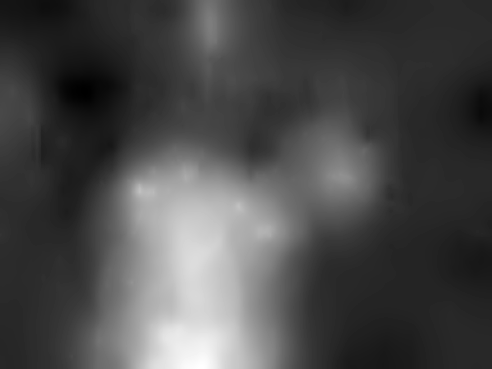
\includegraphics[width=\textwidth]{output3.png}
    \caption{Constant initialization. $\mu, \sigma, \alpha$ = (0, 1.2, 1.0)}
    \label{fig:image1}
  \end{minipage}
  \hfill
  \begin{minipage}[b]{0.45\textwidth}
    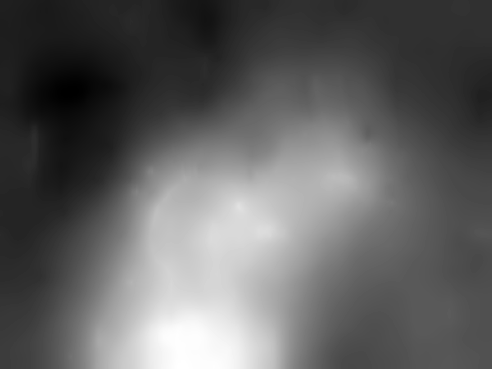
\includegraphics[width=\textwidth]{output4.png}
    \caption{Random initialization. $\mu, \sigma, \alpha$ = (0, 1.2, 1.0)}
    \label{fig:image2}
  \end{minipage}
  \end{figure}
    \begin{figure}[ht]
  \centering
  \begin{minipage}[b]{0.45\textwidth}
    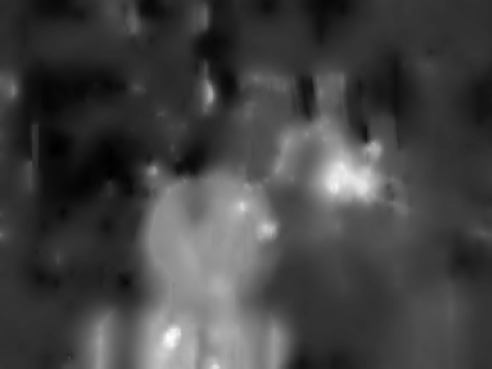
\includegraphics[width=\textwidth]{output5.png}
    \caption{Random initialization. $\mu, \sigma, \alpha$ = (0, 1.2, 0.05)}
    \label{fig:image1}
  \end{minipage}
  \hfill
  \begin{minipage}[b]{0.45\textwidth}
    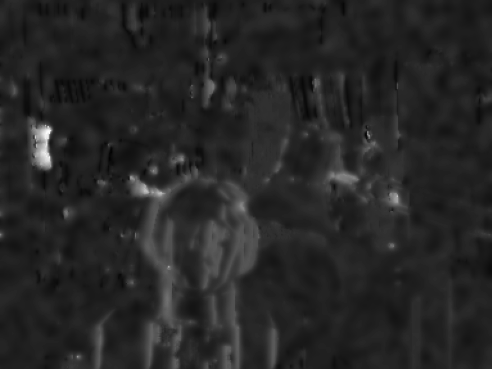
\includegraphics[width=\textwidth]{output6.png}
    \caption{Random initialization. $\mu, \sigma, \alpha$ = (0, 1.2, 0.01)}
    \label{fig:image2}
  \end{minipage}
  \end{figure}
    \begin{figure}[ht]
  \centering
  \begin{minipage}[b]{0.45\textwidth}
    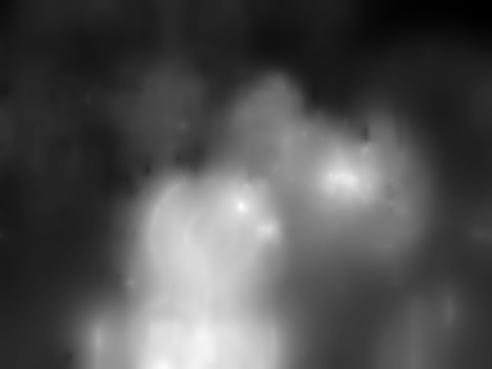
\includegraphics[width=\textwidth]{output7.png}
    \caption{GT initialization (pyramid). $\mu, \sigma, \alpha$ = (0, 1.2, 0.05)}
    \label{fig:image1}
  \end{minipage}
  \hfill
  \begin{minipage}[b]{0.45\textwidth}
    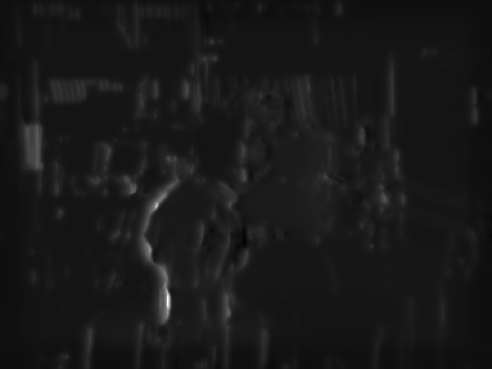
\includegraphics[width=\textwidth]{output9.png}
    \caption{GT initialization. $\mu, \sigma, \alpha$ = (0, 1.2, 0.05)}
    \label{fig:image2}
  \end{minipage}
  \end{figure}
  
	
\end{document}
